\documentclass[10pt,conference]{IEEEtran}
\IEEEoverridecommandlockouts
% The preceding line is only needed to identify funding in the first footnote. If that is unneeded, please comment it out.
\usepackage{CTEX}
\usepackage{cite}
\usepackage{amsmath,amssymb,amsfonts}
\usepackage{algorithmic}
\usepackage{graphicx}
\usepackage{textcomp}
\usepackage{multirow} 
\usepackage{xcolor}
\usepackage{url}

\usepackage{hyperref} % 提供超链接支持
% 设置超链接样式
\hypersetup{
    colorlinks=true,
    linkcolor={red!50!black},   % 深红色（图表引用等）
    citecolor={blue!65!black},  % 深蓝色（参考文献）
    urlcolor={blue!80!black}    % 亮蓝色（网址 URL）
}

\usepackage{booktabs} % 用于 \toprule, \midrule, \bottomrule 绘制三线表
\def\BibTeX{{\rm B\kern-.05em{\sc i\kern-.025em b}\kern-.08em
    T\kern-.1667em\lower.7ex\hbox{E}\kern-.125emX}}
\begin{document}

\title{面向可见光--热红外语义分割的差异引导互补残差融合方法* %
\thanks{*本文为硕士研究生课程《多传感器智能信息融合》课程设计报告}}

\author{%
\IEEEauthorblockN{1\textsuperscript{st} 李奕帆}
\IEEEauthorblockA{\textit{学号：26725496}\\
\textit{上海大学 \quad 未来技术学院}\\
\textit{人工智能专业硕士研究生}\\
Email: yifan-li@shu.edu.cn}

\and


\IEEEauthorblockN{2\textsuperscript{nd} 董义贇}
\IEEEauthorblockA{\textit{学号：26725498}\\
\textit{上海大学 \quad 未来技术学院}\\
\textit{人工智能专业硕士研究生}\\
Email: dyy\_dong@shu.edu.cn}
\and


\IEEEauthorblockN{3\textsuperscript{rd} 宋旭婷}
\IEEEauthorblockA{\textit{学号：26721765}\\
\textit{上海大学 \quad 计算机工程与科学学院}\\
\textit{人工智能专业硕士研究生}\\
Email: 13696672691@163.com}
\and

\IEEEauthorblockN{4\textsuperscript{th} 丁悦}
\IEEEauthorblockA{\textit{学号：26721764}\\
\textit{上海大学 \quad 计算机工程与科学学院}\\
\textit{人工智能专业硕士研究生}\\
Email: joydy2022@163.com}

}



\maketitle

\begin{abstract}
可见光（RGB）与热红外图像在全天候场景理解中具有天然互补性：前者提供丰富的纹理与颜色信息，后者对光照变化不敏感，能稳定刻画行人、车辆等热目标。以 RTFNet 为代表的双流网络通过逐阶段逐元素相加实现融合，结构简洁、训练稳定，但固定的 1:1 合并方式无法显式区分两模态一致与冲突互补的区域。为此，本文提出差异引导互补残差融合（DCR）方法：保留相加融合作为主干通路，并在其上叠加轻量残差校正支路，以两模态归一化特征的绝对差异与共激活响应为输入，经通道与空间注意力调制后，由零初始化的逐通道系数注入融合特征。训练阶段进一步提出差异加权损失（DWL），利用跨模态差异图对像素级分割损失进行归一化重加权。在 MFNet 数据集上，DCR 将测试集 mIoU 由 52.17 提升至 53.75（+1.58）；在七种输入退化条件下，平均 mIoU 由 47.32 提升至 49.10，且在RGB缺失、热红外缺失等七种退化条件下均优于基线；所提出方法仅增加 0.526M 参数（约 2.1\%）与 0.37 GFLOPs。我们的代码已在 \url{https://github.com/nac-max/MultiSensor-DCR} 开源，项目主页为 \url{http://115.191.43.228:8081/}。
\end{abstract}

\begin{IEEEkeywords}
可见光，热红外，语义分割，双流网络，差异引导
\end{IEEEkeywords}

\section{引言}

语义分割是自动驾驶感知的基础任务。仅依赖 RGB 相机的分割模型在夜间、强逆光、雾霾等条件下性能显著下降；热红外相机依据物体自身热辐射成像，对光照不敏感，能够在暗光下稳定呈现行人与车辆。因此，RGB-T 语义分割成为提升全天候感知可靠性的重要方向。MFNet \cite{b1} 首次发布了城市道路场景的 RGB-T 语义分割基准，并给出一个实时双编码器网络；RTFNet \cite{b2} 进一步采用双流 ResNet \cite{b3} 编码器，并在各阶段对两路特征逐元素相加，成为该领域最常用的融合基线之一。

逐元素相加融合的优点在于无额外参数、梯度传播直接、训练稳定；然而它隐含地假设两种模态在任意位置的可靠性相同。实际场景中这一假设经常不成立：白天的路沿与锥桶在 RGB 中纹理清晰，在热红外中却几乎不可见；夜间行人在 RGB 中被暗光淹没，在热红外中轮廓明确；传感器噪声、遮挡或配准误差还会使某一模态在局部失效。此时两模态的特征响应出现差异，而这正是模型需要做出"取舍或互补"判断的位置。后续工作（如 GMNet \cite{b5}、EGFNet \cite{b6}、LASNet \cite{b7}、CMX \cite{b8}）引入了门控、注意力或特征校正机制，但往往以复杂的重加权模块整体替换相加操作，可能破坏相加融合在小数据集上的稳定性。



本文的主要贡献如下：

\begin{enumerate}
    \item 提出 DCR 融合模块。 DCR 以相加融合为恒等主干，利用归一化跨模态差异 $D$ 与共激活响应 $P$ 构造互补残差，并通过通道/空间注意力与零初始化逐通道系数 $\alpha$ 控制注入强度。
    \item 提出差异加权损失 DWL。 以 DCR 产生的差异图对主分割损失进行均值归一化重加权，在不改变总损失尺度的前提下，使优化更多关注跨模态冲突区域。
    \item 开展了较为系统的实验验证。复现了单模态基线和 RTFNet 式相加融合基线，并分析了七种输入退化下的鲁棒性、组件消融与计算开销，并客观讨论方法的失效情形。
\end{enumerate}





\section{相关工作}

GB-T 语义分割方面，MFNet \cite{b1} 提出包含 1569 对已配准 RGB-T 图像的城市场景数据集及轻量双编码器网络，PST900 \cite{b4} 将该任务扩展至地下环境；RTFNet \cite{b2} 以双流 ResNet \cite{b3} 编码器与逐阶段相加融合为核心，在 MFNet \cite{b1} 上取得 51.7（ResNet-50）与 53.2（ResNet-152）mIoU，其简洁性使其成为后续工作最常用的对照基线。然而，这一范式的简洁正源于其固定 1:1 的融合权重：它对两模态一视同仁，无法区分二者一致与冲突的空间位置。 

为引入选择性，GMNet \cite{b5} 采用分层门控与多任务监督，EGFNet \cite{b6} 引入边缘先验引导融合，LASNet \cite{b7} 针对不同层级设计定位、激活与锐化模块，CMX \cite{b8} 提出跨模态特征校正与交叉注意力融合并扩展为通用 RGB-X 框架 CMNeXt \cite{b9}。这类方法表明，自适应调节模态贡献能够提升性能，但其融合模块通常整体替换相加，参数与计算开销较大，且在中小规模数据集上可能因重加权自由度偏高而影响相加融合的训练稳定性。这促使本文采取相反的取舍：保留相加作为不可动摇的主干，仅在残差支路上引入自适应。

与此同时，近期工作开始显式关注模态差异：MDRNet \cite{b12} 从缓解模态差异的角度设计网络，CAINet \cite{b11} 与 EAEFNet \cite{b10} 分别利用上下文交互与显式注意力增强融合，Sigma \cite{b13} 则基于状态空间模型建模跨模态交互。上述方法虽已认识到差异的重要性，但普遍将差异用于构造或替换主融合路径。



\section{方法}

\subsection{整体框架}

本文采用双流编码与共享解码架构，如图~\ref{fig:framework}所示。RGB 与热红外图像分别输入独立的 ResNet-18 编码器提取多尺度特征。编码阶段逐级融合双模态特征：第 1 阶段两模态差异较小，直接采用无参数逐元素相加；第 2 至 4 阶段语义信息丰富，采用 DCR 模块进行精细化校正。融合特征仅馈入解码器，以保障双模态特征提取的独立性。

\begin{figure*}[!t]
\centering
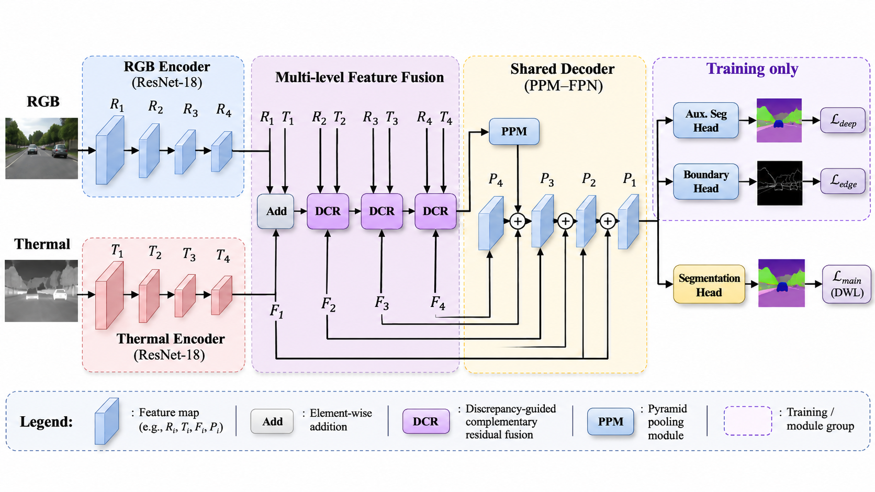
\includegraphics[width=\textwidth]{./figures/整体框架.png}
\caption{整体网络结构。RGB 与热红外图像分别由两个 ResNet-18 编码器提取四个阶段的特征；第 1 阶段采用逐元素相加融合，第 2--4 阶段采用 DCR 融合；融合特征送入共享的 PPM-FPN 解码器输出 9 类分割结果。}
\label{fig:framework}
\end{figure*}

融合后的四级特征送入共享解码器，经金字塔池化聚合全局上下文，并通过自上而下的横向连接融合多尺度语义与细节，最终输出像素级分割结果。训练阶段引入辅助语义头与边界预测头提供额外约束，主损失采用差异加权策略，引导模型聚焦于双模态响应不一致的区域。

\subsection{差异引导互补残差融合模块(DCR)}

DCR 模块流程如图~\ref{fig:dcr}所示。相加融合可视为两路特征的“共识”估计，但在模态冲突时会混合噪声。为此，DCR 采用残差架构：以相加融合为主干保留基础信息，基于跨模态差异与共激活特征构建轻量校正分支，经注意力调制后注入主干，在保证训练稳定性的前提下实现精细化融合。


\begin{figure*}[!t]
\centering
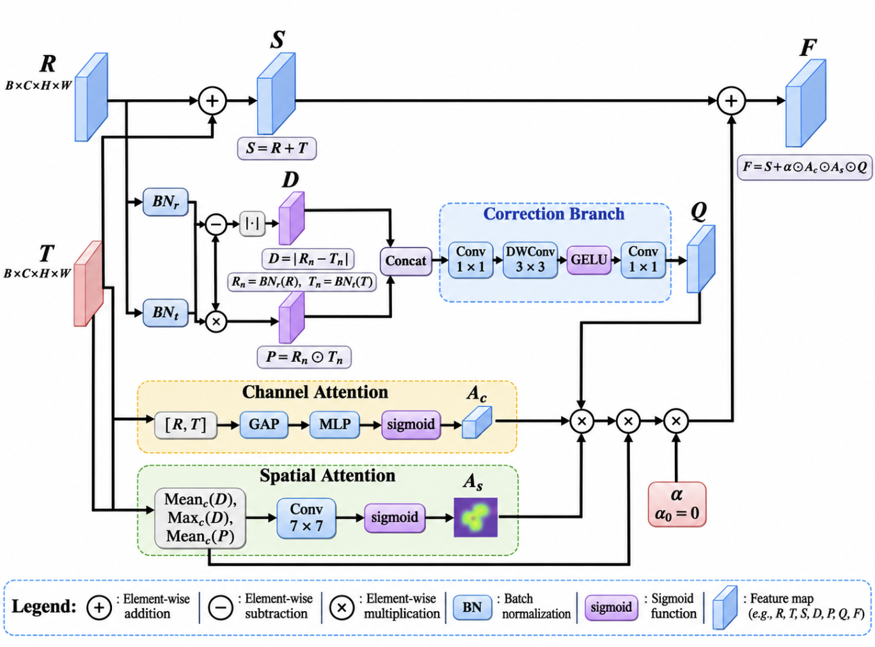
\includegraphics[width=\textwidth]{./figures/DCR.png}
\caption{DCR 模块结构。模块以 $R+T$ 为主干，利用归一化差异 $D$ 与共激活 $P$ 生成残差校正，经通道注意力 $A_c$、空间注意力 $A_s$ 与零初始化系数 $\alpha$ 调制后加回主干。}
\label{fig:dcr}
\end{figure*}

给定同一阶段的 RGB 特征 \(R\) 与热红外特征 \(T\)，主干及跨模态线索计算如下：
\begin{equation}
S = R + T, \quad D = |R_n - T_n|, \quad P = R_n \odot T_n
\end{equation}
其中，\(R_n = \text{BN}_r(R)\) 与 \(T_n = \text{BN}_t(T)\) 为独立批归一化后的特征；\(S\) 为基础融合特征；\(D\) 刻画两模态的空间响应分歧；\(P\) 刻画共激活强度；\(\odot\) 为逐元素乘法。\([D, P]\) 提供了两模态关系的显式二阶描述。

\(D\) 与 \(P\) 拼接后输入校正分支，经 \(1\times1\) 卷积降维、\(3\times3\) 深度卷积提取局部关联，再由 \(1\times1\) 卷积恢复维度，得到残差特征 \(Q\)：
\begin{equation}
\begin{split}
Q = \text{Conv}_{1\times1}\Big\{ \text{GELU}\Big[ & \text{DWConv}_{3\times3} \\
& \left( \text{Conv}_{1\times1}([D, P]) \right) \Big] \Big\}
\end{split}
\end{equation}

为自适应调制校正强度，模块并行计算通道与空间注意力。通道注意力聚合全局上下文生成通道权重 \(A_c\)；空间注意力利用差异与共激活的通道统计量生成空间权重 \(A_s\)：
\begin{equation}
A_c = \sigma\left( \text{MLP}\left( \text{GAP}([R, T]) \right) \right)
\end{equation}
\begin{equation}
A_s = \sigma\left( \text{Conv}_{7\times7}\left( \left[ \text{Mean}_c(D), \text{Max}_c(D), \text{Mean}_c(P) \right] \right) \right)
\end{equation}
其中，\(\sigma\) 为 Sigmoid 函数。最终融合特征为：
\begin{equation}
F = S + \alpha \odot A_c \odot A_s \odot Q
\end{equation}
其中 \(\alpha\) 为逐通道缩放系数且初始化为 \(0\)。该设计确保了训练初始阶段 \(F \equiv S\)，即 DCR 与相加基线严格等价，避免了替换式融合在早期破坏预训练特征的问题。同时，由于 \(Q\) 不为零，\(\alpha\) 可获得有效梯度，使模型能够平稳地学习有益的特征偏离。

\subsection{共享多尺度解码器}

为排除解码端差异干扰，所有对比模型均采用结构相同的 PPM-FPN 解码器，通道宽度统一为 128。解码器接收四级融合特征，通过多尺度金字塔池化聚合全局上下文，并利用自上而下的横向连接融合多尺度语义与细节，最终统一上采样至输入分辨率。最终聚合特征分别连接主语义分割头与单通道边界预测头，同时在第 3 阶段特征上设置辅助语义头以提供深监督。所有预测结果经双线性插值恢复原始大小参与损失计算。

\subsection{类别加权与差异加权损失}

针对 MFNet 的类别不平衡问题，本文在主损失中引入类别加权，并结合跨模态差异设计差异加权损失（DWL）。设类别频率为 \(f_c\)，类别权重 \(w_c\) 定义为：
\begin{equation}
\tilde{w}_{c}=\frac{1}{\ln{\left(1.10+f_{c}\right)}},\quad w_{c}=\frac{\tilde{w}_{c}}{K^{-1}\sum_{j=1}^{K} \tilde{w}_{j}}
\end{equation}

DWL 根据特征差异调整像素权重。取第 2 阶段差异特征 \(D\) 沿通道求均值，经最小–最大归一化并上采样至标签分辨率得到 \(M\)：
\begin{equation}
\begin{split}
d &= {\text{Mean}}_{c}\left(D\right), \\
M &= \text{stopgrad}\left[\text{Resize}\left(\frac{d-\min{\left(d\right)}}{\max{\left(\max{\left(d\right)}-\min{\left(d\right)},\varepsilon \right)}}\right)\right]
\end{split}
\end{equation}
其中 \(\varepsilon=10^{-6}\) 防止除零。`stopgrad` 操作切断了梯度向编码器的回传，防止网络通过刻意压低差异来逃避惩罚，确保差异响应是特征的自然输出。

设 \(V\) 为有效像素集合，先计算像素权重 \(q_i\) 并做均值归一化得到 \(\bar{q}_i\)，以保持总体损失尺度不变：
\begin{equation}
q_{i}=1+\beta M_{i},\quad \bar{q}_{i}=\frac{q_{i}}{{\left|V\right|}^{-1}\sum_{j\in V} q_{j}}
\end{equation}
结合类别权重，最终的主分割损失为：
\begin{equation}
\mathcal{L}_{main}=\frac{\sum_{i\in V} w_{y_{i}}\bar{q}_{i}\left[-\ln{p}_{i}\left(y_{i}\right)\right]}{\sum_{i\in V} w_{y_{i}}}
\end{equation}
其中 \(\beta=1\)，\(y_i\) 为真实类别，\(p_i\) 为预测概率。当 \(\beta=0\) 时，DWL 退化为纯类别加权交叉熵。

\subsection{深监督与边界监督}

第 3 阶段的辅助语义头采用类别加权交叉熵提供深监督。边界监督由真值直接构造：若像素 \(i\) 的 \(3\times3\) 邻域内存在类别不同的有效像素，则记为边界：
\begin{equation}
b_{i}=\mathbb{1}\left[i\in V \wedge \exists j\in \mathcal{N}_{3\times 3}\left(i\right)\cap V:\ y_{i}\neq y_{j}\right]
\end{equation}
边界损失 \(\mathcal{L}_{edge}\) 采用加权二值交叉熵，正类权重按批次统计自适应设为 \(\min{\left(N_{neg}/N_{pos},20\right)}\) 以缓解样本失衡。

\subsection{总体训练目标}

总损失由主语义损失、深监督损失与边界损失加权构成：
\begin{equation}
\mathcal{L}={\mathcal{L}}_{main}+0.4{\mathcal{L}}_{deep}+0.5{\mathcal{L}}_{edge}
\end{equation}
其中，完整 DCR 模型使用含 DWL 的 \(\mathcal{L}_{main}\)，而基线与消融模型退化为纯类别加权交叉熵。除 DWL 外，所有损失项及系数在基线间完全一致，确保对比公平。

%%%%%%%%%%%%%%%%%%%%%%

\section{实验设置}

\subsection{数据集}

实验采用 Ha 等人[1]构建的 MFNet 城市场景数据集，共包含 1569 对已配准的可见光与热红外图像。数据涵盖汽车、行人、自行车、弯道、停车线、护栏、锥形筒与减速带等 9 个类别。官方划分包含 784 幅训练图、392 幅验证图与 393 幅测试图，各子集之间无图像重叠；其中测试集由 205 幅白天图像与 188 幅夜间图像构成。预处理时，标签值为 0 的未标注区域作为背景类参与训练与评估，仅标签值为 255 的像素作为忽略项不参与计算。

每个数据样本为四通道图像，前三个通道为可见光图像，第四个通道为热红外图像。可见光图像经归一化至 \([0, 1]\) 区间后，采用 ImageNet 的均值与标准差进行标准化处理；热红外图像则被映射至 \([-1, 1]\) 区间以适配网络输入。为提升模型的泛化能力与鲁棒性，训练阶段引入了随机缩放、随机裁剪与随机水平翻转等数据增强策略；测试阶段则统一采用确定性预处理，确保评估结果的公平性与可复现性

\subsection{评价指标}

分割性能采用交并比（IoU）与平均交并比（mIoU）进行评估。针对每个测试子集，统计所有图像的像素级混淆矩阵后，计算各类别的 IoU 及 mIoU：
\begin{equation}
\mathrm{IoU}_{c} = \frac{\mathrm{TP}_{c}}{\mathrm{TP}_{c} + \mathrm{FP}_{c} + \mathrm{FN}_{c}}, \quad \mathrm{mIoU} = \frac{1}{|C|} \sum_{c \in C} \mathrm{IoU}_{c}
\end{equation}
其中，\(\mathrm{TP}_{c}\)、\(\mathrm{FP}_{c}\) 与 \(\mathrm{FN}_{c}\) 分别表示类别 \(c\) 的真正例、假正例与假负例的像素数；\(C\) 为预测或标注中至少出现一次的类别集合，\(|C|\) 为该集合的基数。

针对模型鲁棒性，采用 7 种输入退化条件下的平均 mIoU 及其相对无扰动测试集的降幅进行衡量。设 \(m_{k}\) 为第 \(k\) 种退化条件下的 mIoU，\(m_{\mathrm{clean}}\) 为无扰动测试集上的 mIoU，则：
\begin{equation}
m_{\deg} = \frac{1}{7} \sum_{k=1}^{7} m_{k}, \quad \Delta_{\mathrm{drop}} = m_{\mathrm{clean}} - m_{\deg}
\end{equation}
降幅 \(\Delta_{\mathrm{drop}}\) 以百分点为单位计。对于采用 3 个随机种子的所有实验，最终结果以均值 \(\pm\) 样本标准差（\(\mu \pm \sigma\)）的形式说明。


\section{实验结果与讨论}

\subsection{公开基线复现与对比}

表~\ref{tab:main_results_mega} 汇总了本文方法、复现基线以及公开方法在 MFNet 测试集上的综合表现，涵盖整体 mIoU、昼夜子集以及 9 类逐类 IoU。


\begin{table*}[!t]
\centering
\caption{MFNet 测试集上的综合性能对比（mIoU，\%）。† 表示引自原论文；其余为本文统一代码复现。Day/Night 为昼夜子集，右侧为 9 类逐类 IoU。}
\label{tab:main_results_mega}
\resizebox{\textwidth}{!}{
\begin{tabular}{lllcccccccccccc}
\toprule
\multirow{2}{*}{方法} & \multirow{2}{*}{骨干} & \multirow{2}{*}{解码器 / 配置} & \multirow{2}{*}{mIoU} & \multicolumn{2}{c}{子集} & \multicolumn{9}{c}{逐类 IoU} \\
\cmidrule(lr){5-6} \cmidrule(lr){7-15}
 & & & & Day & Night & Unlab & Car & Per & Bike & Curv & Stop & Guar & Cone & Bump \\
\midrule
MFNet† [1] & 轻量 CNN & 原文解码器 & 33.70 & - & - & - & - & - & - & - & - & - & - & - \\
RTFNet-50† [2] & ResNet-50 & Upception (原文) & 51.70 & - & - & - & - & - & - & - & - & - & - & - \\
RTFNet-152† [2] & ResNet-152 & Upception (原文) & 53.20 & - & - & - & - & - & - & - & - & - & - & - \\
\midrule
RGB-only & ResNet-18 & 基础配置 & 49.96 & 45.27 & 48.13 & - & - & - & - & - & - & - & - & - \\
Thermal-only & ResNet-18 & 基础配置 & 46.68 & 38.93 & 48.26 & - & - & - & - & - & - & - & - & - \\
RTFNet-style & ResNet-18$\times$2 & 基础配置 & 52.01 & 45.87 & 51.67 & - & - & - & - & - & - & - & - & - \\
\midrule
Add. Baseline & ResNet-18$\times$2 & PPM-FPN + 辅助损失 & 52.17 & 45.18 & 52.82 & 97.23 & 83.67 & 69.24 & 57.14 & 35.39 & 29.42 & 4.77 & 47.46 & 45.23 \\
\textbf{DCR + DWL (本文)} & ResNet-18$\times$2 & PPM-FPN + 辅助损失 & \textbf{53.75} & \textbf{47.02} & \textbf{53.77} & \textbf{97.53} & \textbf{85.55} & \textbf{70.11} & \textbf{59.87} & \textbf{38.35} & \textbf{30.64} & 4.50 & \textbf{49.98} & \textbf{47.21} \\
\midrule
\textbf{绝对增益} & - & - & \textbf{+1.58} & +1.84 & +0.95 & +0.30 & +1.88 & +0.87 & +2.73 & +2.96 & +1.22 & -0.27 & +2.52 & +1.98 \\
\bottomrule
\multicolumn{15}{l}{\footnotesize 注：Unlab=未标注, Per=行人, Curv=弯道, Stop=停车挡块, Guar=护栏, Cone=彩色锥桶, Bump=减速带。}
\end{tabular}}
\end{table*}

\textbf{基线复现与公平对比。} 我们首先复现了 RTFNet 式的逐阶段相加融合基线。需要指出的是，RTFNet 原文采用其专门设计的 Upception 解码器。为在统一的实验条件下隔离融合模块的影响，本文在复现时未采用 Upception，而是借鉴了 UPerNet \cite{b14}等工作的思路，构建了一个由金字塔池化模块（PPM）与特征金字塔网络（FPN）组成的标准多尺度解码器，并将其作为所有对比模型（含基线与本文方法）的公共底座。在基础配置下，RTFNet 式相加融合达到了 52.01\% 的 mIoU，与 RTFNet-50 原文报告值（51.70\%）基本持平，验证了本文训练评测流程的可靠性。

此外，单模态实验表明，热红外在夜间（48.26\%）表现优异，但在白天（38.93\%）显著弱于 RGB（45.27\%），证明了多模态融合的必要性。为了严格评估 DCR 的收益，我们构建了强化相加基线（Add. Baseline），为其配备了与完整模型完全相同的 PPM-FPN 解码器、深监督与边界损失。结果显示，该基线 mIoU 提升至 52.17\%，较基础配置仅有微弱提升（+0.16\%）。这一控制变量设计证明：解码器与辅助损失的增强本身并不能带来显著收益，从而确保了后续 DCR 的性能增益可被唯一归因于融合策略本身的改进。

\textbf{整体性能与稳定性。} DCR+DWL 将整体 mIoU 提升至 \textbf{53.75\%}（+1.58\%），在参数量远小于 RTFNet-152 的前提下，达到了与其原文报告值（53.20\%）相当的性能水平。跨三个随机种子的实验表明，DCR 在最差种子下的结果（53.20\%）仍高于基线在最好种子下的结果（52.52\%），且显著降低了模型在白天场景下的跨种子波动（标准差从 1.48 降至 0.30），证明差异驱动的校正不仅提升了精度，还大幅增强了训练稳定性。

\textbf{昼夜场景与逐类分析。} DCR 在白天场景的提升（+1.84\%）显著高于夜间（+0.95\%）。白天热红外对路面等冷目标响应缺失，导致两模态分歧增大，相加融合易将有效 RGB 特征与无效热红外特征等量混合；DCR 通过显式差异图感知到这一冲突并施加残差校正，从而有效缓解了单模态失效问题。逐类结果（表~\ref{tab:main_results_mega} 右侧）印证了这一设计动机：提升最大的弯道（+2.96\%）、自行车（+2.73\%）和彩色锥桶（+2.52\%）均属于高度依赖 RGB 纹理或跨模态轮廓配合的“差异显著目标”。唯一出现下降的类别为护栏（-0.27\%），其主要原因是该类别在训练集中极度长尾（两模型 IoU 均低于 5\%），融合策略的改变难以弥补样本匮乏。



\subsection{传感器退化条件下的鲁棒性}

表~\ref{tab:robustness} 展示了在 7 种模拟传感器退化条件下的测试结果（三种子均值）。DCR 在全部 7 种条件下均优于基线，平均 mIoU 提升 1.77\%。

\textbf{噪声与局部扰动。} 在高斯噪声条件下（RGB 噪声 +2.71\%，热红外噪声 +3.00\%），DCR 展现出最强的鲁棒性优势。由于噪声会使受污染模态的特征分布发生全局偏移，导致跨模态分歧 \(D\) 增大；DCR 能够感知该全局差异并在残差支路上抑制噪声模态的响应，有效避免了相加融合中被动混合噪声的缺陷。同时，DCR 显著降低了不同随机种子下的结果波动（例如热红外噪声下的标准差从 1.61 降至 0.18），表明其鲁棒性不依赖于特定的随机初始化。

\textbf{模态缺失的局限性。} 在热红外缺失时 DCR 增益为 +2.26\%，但在 RGB 模态完全缺失时，DCR 的增益仅为 0.64\%，且存在较大的种子间波动。我们推测，完整模态缺失导致特征分布发生剧烈偏移，差异图 \([D, P]\) 的语义表征部分失效；虽然训练中使用了小概率（5\%）的模态置零增强，但不足以使模型在该极端条件下稳定收敛，这也是本文方法目前的局限之一。

\begin{table}[t]
\centering
\caption{七种模拟退化条件下的测试集 mIoU（\%，三种子均值）。}
\label{tab:robustness}
\resizebox{\columnwidth}{!}{
\begin{tabular}{lccc}
\toprule
条件 & Add. Baseline & DCR + DWL & 增益 \\
\midrule
干净测试集 & 52.17 & 53.75 & +1.58 \\
RGB 缺失 & 41.38 & 42.02 & +0.64 \\
热红外缺失 & 45.26 & 47.52 & +2.26 \\
RGB 噪声 (\(\sigma=0.1\)) & 48.40 & 51.10 & +2.71 \\
热红外噪声 (\(\sigma=0.1\)) & 48.77 & 51.77 & +3.00 \\
热红外平移 (10 px) & 49.82 & 51.36 & +1.53 \\
RGB 遮挡 (25\%) & 46.88 & 48.15 & +1.27 \\
RGB 暗光 ($\times$0.2) & 50.76 & 51.75 & +0.99 \\
\midrule
七种退化平均 & 47.32 & 49.10 & +1.77 \\
\bottomrule
\end{tabular}}
\end{table}

\subsection{消融实验}

为验证 DCR 各组件的具体贡献，我们以随机种子 42 进行了组件消融实验（表~\ref{tab:ablation}）。

\textbf{残差校正范式是核心增益来源。} 所有 DCR 变体的干净 mIoU 与退化平均均高于基线。即使去掉任意一个组件，“相加主干 + 零初始化残差校正”的基础架构仍能带来至少 1.06\% 的干净提升和 1.38\% 的退化提升，说明性能增益的主体来自残差校正的范式创新。

\textbf{显式差异输入是鲁棒性的关键。} 将校正支路的输入由 \([D, P]\) 替换为原始特征拼接 \([R, T]\) 后，干净集仅下降 0.24\%，但在退化条件下平均下降 1.62\%。这表明：在干净数据上，网络可以从原始特征中隐式学到模态交互关系；但在模态发生退化时，显式的 \([D, P]\) 表征能够更直接地暴露特征异常，从而维持模型的鲁棒性。



\textbf{DWL 兼顾精度与鲁棒性。} 去除 DWL 后，干净 mIoU 下降 0.53\%，退化平均下降 1.57\%。强调跨模态分歧区域的优化策略，能够显著改善模型在困难场景下的判别力。

\begin{figure*}[!htbp]
\centering
% 请替换为你实际的图片文件名
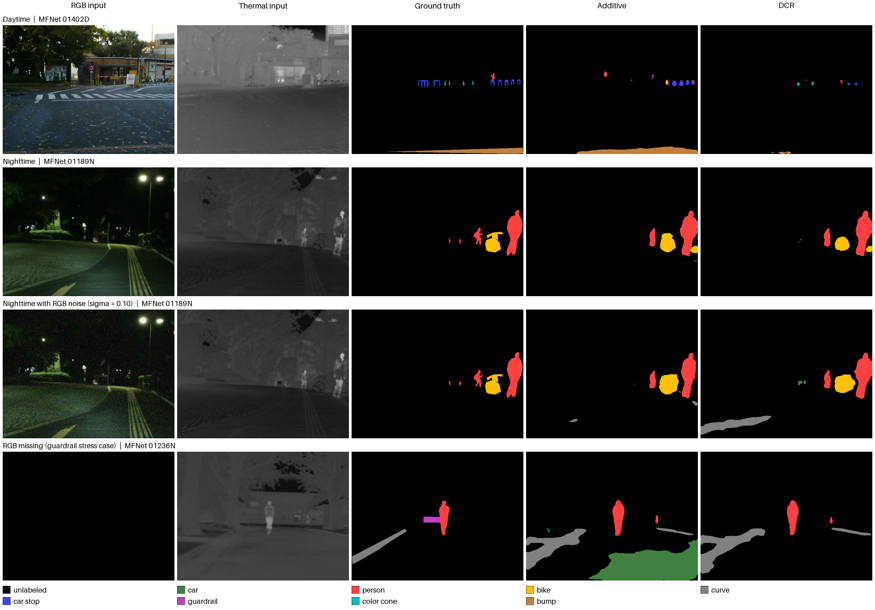
\includegraphics[width=\textwidth]{./figures/可视化.png}
\caption{不同场景及传感器退化条件下的语义分割结果对比。}
\label{fig:qualitative}
\end{figure*}

\textbf{空间注意力作为辅助组件。} 去除空间注意力后，干净集仅下降 0.18\%，但在 RGB 噪声下下降 3.43\%。诊断显示，空间注意力权重 \(A_s\) 在干净图像上均值接近 1（0.99+），说明它倾向于在输入退化引发局部异常时才进行干预。

\begin{table}[t]
\centering
\caption{组件消融实验（seed 42，测试集 mIoU，\%）。}
\label{tab:ablation}
\resizebox{\columnwidth}{!}{
\begin{tabular}{lcccc}
\toprule
配置 & 干净 & 退化平均 & RGB噪声 & 热红外噪声 \\
\midrule
Add. Baseline & 51.61 & 46.10 & 47.62 & 46.92 \\
DCR w/o DWL & 52.67 & 47.53 & 49.44 & 49.68 \\
DCR w/o 空间注意力 & 53.02 & 47.56 & 47.84 & 49.44 \\
DCR w/ 原始 \([R, T]\) & 52.96 & 47.48 & 48.55 & 51.33 \\
\textbf{DCR + DWL (完整)} & \textbf{53.20} & \textbf{49.10} & \textbf{51.27} & \textbf{51.64} \\
\bottomrule
\end{tabular}}
\end{table}

\subsection{可视化分析}

图~\ref{fig:qualitative} 展示了模型在典型场景及传感器退化条件下的分割结果对比。在白天样本中，图像底部的减速带在相加基线结果中基本连续，而 DCR 仅分割出一小段，这与减速带（bump）类在部分种子下的 IoU 表现一致。在夜间样本中，两种模型在无干扰及 RGB 加噪前后均能准确分割出右侧较大的行人，但对远处小目标的分割均不完整；当加入高斯噪声后，DCR 出现将图像左下方区域误分为弯道（curve）的情况。

总体而言，尽管 DCR 在输入退化条件下的统计平均 mIoU 显著高于基线，但定性结果直观地表明，局部误分现象依然存在。统计层面的整体提升并不意味着模型在每一个具体样本上都能做到绝对完美的分割。

\subsection{计算开销分析}

表~\ref{tab:complexity} 对比了基线模型与 DCR 的模型复杂度与推理效率。由于 DCR 仅在第 2–4 阶段引入轻量级的瓶颈卷积与注意力分支，其参数量仅增加 0.526M（2.1\%），计算量（FLOPs）仅增加 0.37G（0.5\%），峰值显存增加 3.3MB，资源占用处于极低水平。

在 RTX 5070 Ti Laptop GPU（输入尺寸 \(480\times640\)，batch size 为 1，FP32 精度）上，DCR 的推理速度达到 105.2 FPS。相较于基线，推理延迟增加了 1.75 ms（速度下降 18.4\%），主要归因于逐元素运算及注意力机制带来的额外显存访问开销。尽管存在这一开销，DCR 仍能保持 105 FPS 以上的推理速度，能满足自动驾驶场景下全天候实时语义分割的需求。


\begin{table}[t]
\centering
\caption{模型复杂度与推理效率对比（\(480\times640\)，batch size 1，FP32）。}
\label{tab:complexity}
\resizebox{\columnwidth}{!}{
\begin{tabular}{lccc}
\toprule
模型 & 参数量 (M) & GFLOPs & FPS \(\uparrow\) \\
\midrule
Add. Baseline & 25.03 & 75.18 & 129.0 \\
\textbf{DCR + DWL (本文)} & \textbf{25.56} & \textbf{75.55} & \textbf{105.2} \\
\midrule
增量 & +0.526 (+2.1\%) & +0.37 (+0.5\%) & -23.8 \\
\bottomrule
\end{tabular}}
\end{table}


\section{结论与讨论}

\subsection{结论}
针对 RGB-T 语义分割中逐元素相加融合无法区分跨模态一致与冲突区域的问题，本文提出了差异引导互补残差融合（DCR）模块与差异加权损失（DWL）。DCR 以相加融合作为恒等主干以保留基础信息，利用归一化特征的绝对差异与共激活响应构建残差校正分支，并通过零初始化的逐通道系数确保训练初期的输出与相加基线严格等价。在此基础上，DWL 通过跨模态差异图对像素级损失进行重加权，引导模型聚焦于模态分歧区域。在统一的代码框架下，本文构建了控制变量严格的强化公平基线。三个随机种子的实验表明，DCR 将 MFNet 测试集的 mIoU 稳定提升了 1.58\%，且在七种模拟传感器退化条件下全面优于基线（平均提升 1.77\%），同时显著降低了跨随机种子的方差，且仅增加了 2.1\% 的参数量与极小的推理延迟。


\subsection{局限性}
尽管 DCR 在受控实验中表现优异，本文方法仍存在以下局限：（1）在完整 RGB 模态缺失的极端条件下，DCR 的增益不稳定且跨种子波动较大，表明模型对剧烈特征分布偏移的适应能力仍有待提升；（2）对于 \textit{guardrail} 等极稀有类别，分割性能依然处于极低水平，未来需结合数据重采样或长尾损失函数进行专项优化；（3）目前仅在 MFNet 单一数据集上进行了验证，尚未在 PST900 等其他 RGB-T 数据集上测试其泛化能力。


\subsection{未来工作}

未来工作将聚焦于以下三个方向：一是探索更先进的模态缺失模拟与训练策略，以提升极端退化条件下的鲁棒性；二是引入长尾学习机制以改善稀有类别的分割质量；三是将 DCR 推广至 Transformer 或 Mamba 等更强骨干网络，并在更多样化的多传感器数据集（如 PST900）上验证其泛化性能。






































\begin{thebibliography}{99}

\bibitem{b1} Q. Ha, K. Watanabe, T. Karasawa, Y. Ushiku, and T. Harada, ``MFNet: Towards real-time semantic segmentation for autonomous vehicles with multi-spectral scenes,'' in \textit{Proc. IEEE/RSJ Int. Conf. Intell. Robots Syst. (IROS)}, 2017.

\bibitem{b2} Y. Sun, W. Zuo, and M. Liu, ``RTFNet: RGB-thermal fusion network for semantic segmentation of urban scenes,'' \textit{IEEE Robot. Autom. Lett.}, vol. 4, no. 3, pp. 2576--2583, 2019.

\bibitem{b3} K. He, X. Zhang, S. Ren, and J. Sun, ``Deep residual learning for image recognition,'' in \textit{Proc. IEEE Conf. Comput. Vis. Pattern Recognit. (CVPR)}, 2016, pp. 770--778.

\bibitem{b4} S. S. Shivakumar, N. Rodrigues, A. Zhou, I. D. Miller, V. Kumar, and C. J. Taylor, ``PST900: RGB-thermal calibration, dataset and segmentation network,'' in \textit{Proc. IEEE Int. Conf. Robot. Autom. (ICRA)}, 2020, pp. 9441--9447.

\bibitem{b5} W. Zhou, J. Liu, J. Lei, L. Yu, and J.-N. Hwang, ``GMNet: Graded-feature multilabel-learning network for RGB-thermal urban scene semantic segmentation,'' \textit{IEEE Trans. Image Process.}, vol. 30, pp. 7790--7802, 2021.

\bibitem{b6} S. Dong, W. Zhou, C. Xu, and W. Yan, ``EGFNet: Edge-aware guidance fusion network for RGB-thermal urban scene parsing,'' \textit{IEEE Trans. Intell. Transp. Syst.}, 2023.

\bibitem{b7} G. Li, Y. Wang, Z. Liu, X. Zhang, and D. Zeng, ``RGB-T semantic segmentation with location, activation, and sharpening,'' \textit{IEEE Trans. Circuits Syst. Video Technol.}, vol. 33, no. 3, pp. 1223--1235, 2023.

\bibitem{b8} J. Zhang, H. Liu, K. Yang, X. Hu, R. Liu, and R. Stiefelhagen, ``CMX: Cross-modal fusion for RGB-X semantic segmentation with transformers,'' \textit{IEEE Trans. Intell. Transp. Syst.}, vol. 24, no. 12, pp. 14679--14694, 2023.

\bibitem{b9} J. Zhang, R. Liu, H. Shi, K. Yang \textit{et al.}, ``Delivering arbitrary-modal semantic segmentation,'' in \textit{Proc. IEEE/CVF Conf. Comput. Vis. Pattern Recognit. (CVPR)}, 2023.

\bibitem{b10} M. Liang, J. Hu, C. Bao, H. Feng, F. Deng, and T. L. Lam, ``Explicit attention-enhanced fusion for RGB-thermal perception tasks,'' \textit{IEEE Robot. Autom. Lett.}, vol. 8, no. 8, pp. 4606--4613, 2023.

\bibitem{b11} Y. Lv, Z. Liu, and G. Li, ``Context-aware interaction network for RGB-T semantic segmentation,'' \textit{IEEE Trans. Multimedia}, 2024.

\bibitem{b12} S. Zhao, Y. Liu, Q. Jiao, Q. Zhang, and J. Han, ``Mitigating modality discrepancies for RGB-T semantic segmentation,'' \textit{IEEE Trans. Neural Netw. Learn. Syst.}, 2023.

\bibitem{b13} Z. Wan, P. Zhang, Y. Wang, S. Yong, S. Stepputtis, K. Sycara, and Y. Xie, ``Sigma: Siamese Mamba network for multi-modal semantic segmentation,'' in \textit{Proc. IEEE/CVF Winter Conf. Appl. Comput. Vis. (WACV)}, 2025.

\bibitem{b14} T. Xiao, Y. Liu, B. Zhou, Y. Jiang, and J. Sun, ``Unified perceptual parsing for scene understanding,'' in \textit{Proc. Eur. Conf. Comput. Vis. (ECCV)}, 2018, pp. 418--434.
\end{thebibliography}

\end{document}